\documentclass{beamer}
\usepackage[british]{babel}
\usepackage[utf8]{inputenc}
\usepackage{styles/jyumacros}
\usepackage[version=4]{mhchem}
\usepackage{textgreek}
\usefolder{styles}
\usetheme{jyu}

%change these to your own logos if needed (try and match sizes, otherwise, change sizes in Outer Theme file).
\titlegraphic{assets/coverlogo.pdf} %logo on the cover page
\newcommand{\smalllogo}{assets/small_white.pdf} %small logo on frames

%Personal info---------------------------------------------
\title{Journal Club}
\subtitle{Identification of the New Isotope \ce{^{244}Md}\\ J.L.~Pore~\textit{et al.}, PRL\textbf{124} (2020) 252502}
\date{6.7.2021}
\author[auth]{Jorge Romero}
\institute[inst]{Jyväskylän Yliopisto}
%----------------------------------------------------------

\begin{document}
\begin{frame}
\titlepage
\end{frame}

\begin{frame}{Motivation}
    \begin{itemize}
        \item Increasing the known data on isotopes in the Z$\sim$100 region.
    \end{itemize}
\end{frame}
\begin{frame}{Setup}
    \centering
    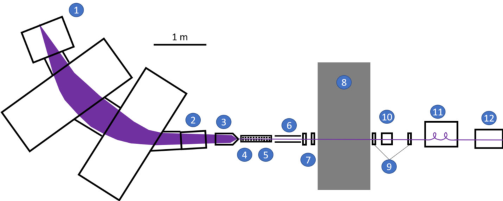
\includegraphics{assets/Fiona.pdf}\\
    BGS (Berkley Gas-filled Separator)  + FIONA (For the Identification Of Nuclide A)\\
    Mass number identification resolving power of 250 at FW-tenth-M  
    
\end{frame}
\begin{frame}{Reaction}
    \begin{center}
        \textbf{\ce{^{209}Bi( ^{40}Ar, 5n) ^{244}Md}}\\
        \ce{^{40}Ar^{9+}} at 220\,MeV and 15\,e\textmu A \\
        0.5\,mg/cm$^2$ \ce{^{209}Bi} target.
    \end{center}
$\color{secondary}{\blacktriangleright}$ Calibration:
\begin{center}
    \ce{^{209}Bi( ^{40}Ar, 2n) ^{247}Md}\\
    \ce{^{165}Ho( ^{40}Ar, 4-6n) ^{199-201}Md}
\end{center}
$\color{secondary}{\blacktriangleright}$ Rescaling:
\begin{center}
    $\left[\frac{(A/q)_{new}}{(A/q)_{cal}}\right]_{244} = 0.6162$\hspace{2em} $\left[\frac{(A/q)_{new}}{(A/q)_{cal}}\right]_{245}=0.6187$
\end{center}
\end{frame}

\begin{frame}{Controversy}
    \vspace{1.2em}
    "In such studies, several neighboring isotopes of a given element can be created simultaneously from the different exit channels of a single nuclear reaction. It is not uncommon for neighboring isotopes to have similar decay properties, which can make it a challenge to assign decay properties to a specific isotope." 
    \vfill
    "the energy and correlation time of the first \textalpha\ in this event are different than decays assigned to \ce{^{244}Md} in events 3, 4, 5, and 6 [...]. Therefore, the first \textalpha\ is tentatively assigned as the decay of a longer-lived isomeric state in \ce{^{244}Md}. Such states have been observed in the neighboring neutron-deficient Md isotopes."
\end{frame}
\begin{frame}{Remarks}
    \begin{center}
        \textbf{F.P.~He\ss berger {et al.} PRL 126 (2021) 182501}
    \end{center}
    The findings in the paper conflict with those in Khuyagbaatar et al. PRL 125 (2020) 142504. Additionally, the data is similar to that published for \ce{^{245m}Md}.


\end{frame}
\end{document}